\documentclass[a4paper,12pt]{article}
\usepackage{polski}
\usepackage[utf8]{inputenc}
\usepackage[OT4]{fontenc}
\usepackage{mathtools}
\usepackage{float}
\usepackage{graphicx}
\usepackage{multirow}

\newcommand{\h}[1]{\noindent \bf #1 \rm \\ \noindent}
\newcommand{\italic}[1]{\it #1 \rm}

\begin{document}

\begin{center}
	\LARGE
	Struktury Danych i Złożoność Obliczeniowa \\
	\large
	ĆWICZENIA 2 
\end{center}
\vspace{1cm}

\h{Kopiec:}
Kopiec to drzewo binarne, czyli takie, gdzie każdy rodzic ma maksymalnie 2 potomków. W kopcu wszystkie poziomy głębokości poza ostatnim są w pełni wypełnione. Ostatni poziom głębokości zawsze jest dosunięty do lewej strony.\\

\noindent
Istnieją dwa rodzaje kopców:
\begin{itemize}
	\item \italic{Maksymalny} - gdzie wartość rodzica jest większa lub równa wartości potomków
	\item \italic{Minimalny} - gdzie wartość rodzica jest mniejsza lub równa wartości potomków
\end{itemize}
\vspace{5mm}

\noindent
Element w pierwszym rzędzie nazywamy korzeniem kopca. Kopiec najczęściej jest stosowany jako kolejka priorytetowa, gdzie chcemy mieć szybki dostęp do maksymalnego/minimalnego elementu.\\

\begin{figure}[H]
	\centering
	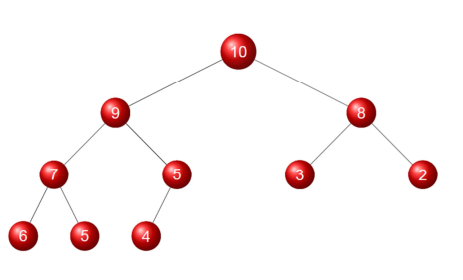
\includegraphics[width=10cm]{fig1.png}
\end{figure}

\h{Złożoności dla kopca:}
\begin{itemize}
	\item \italic{Dodawanie elementu} - $O(\log n)$
	\item \italic{Usuwanie elementu} - $O(\log n)$
	\item \italic{Tworzenie kopca} - $O(n\log n)$ lub $O(n)$ dla algorytmu Floyda
	\item \italic{Wyszukiwanie} - $O(n\log n)$, bo musimy zdejmować z kopca elementy, aż do znalezienia
\end{itemize}
\vspace{5mm}

\h{Dodawanie do kopca:}
Dodawanie do kopca polega na włożeniu elementu na pierwszą wolną pozycję w ostatnim rzędzie. Następnie przeprowadzamy naprawę kopca w górę, aby przywrócić odpowiednie zależności między rodzicami a potomkami. W związku z wymogiem naprawy kopca operacja dodania elementu ma złożoność: $O(\log n)$.\\

\h{Usuwanie z kopca:}
W miejsce usuniętego elementu wstawiamy ostatni dodany do kopca element. Następnie naprawiamy kopiec w dół.\\

\h{Implementacja kopca w tablicy:}
Najpopularniejszy sposób komputerowej implementacji kopca. Taka reprezentacja ma pewne ciekawe zależności między indeksami swoich elementów:
\begin{center}
	\italic{INDEKS RODZICA}\\
	$r = [ \frac{1}{2}(i-1) ]$ \\
	\vspace{5mm}
	\italic{INDEKSY POTOMKÓW}\\
	$p_1 = 2i+1$ lub $p_2 = 2i+2$
\end{center}

\newpage
\h{Algorytm dodawania elementu:}
\begin{figure}[H]
	\centering
	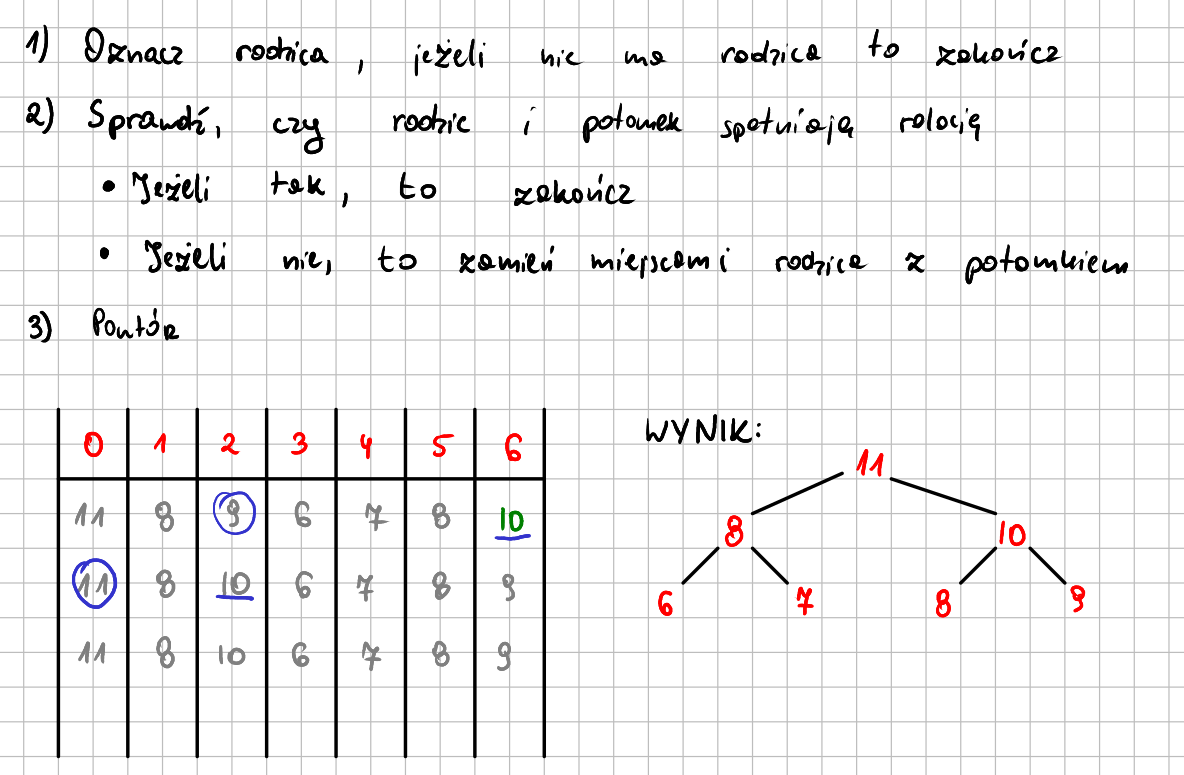
\includegraphics[width=14cm]{fig2.png}
\end{figure}

\newpage
\h{Algorytm usuwania elementu:}
\begin{figure}[H]
	\centering
	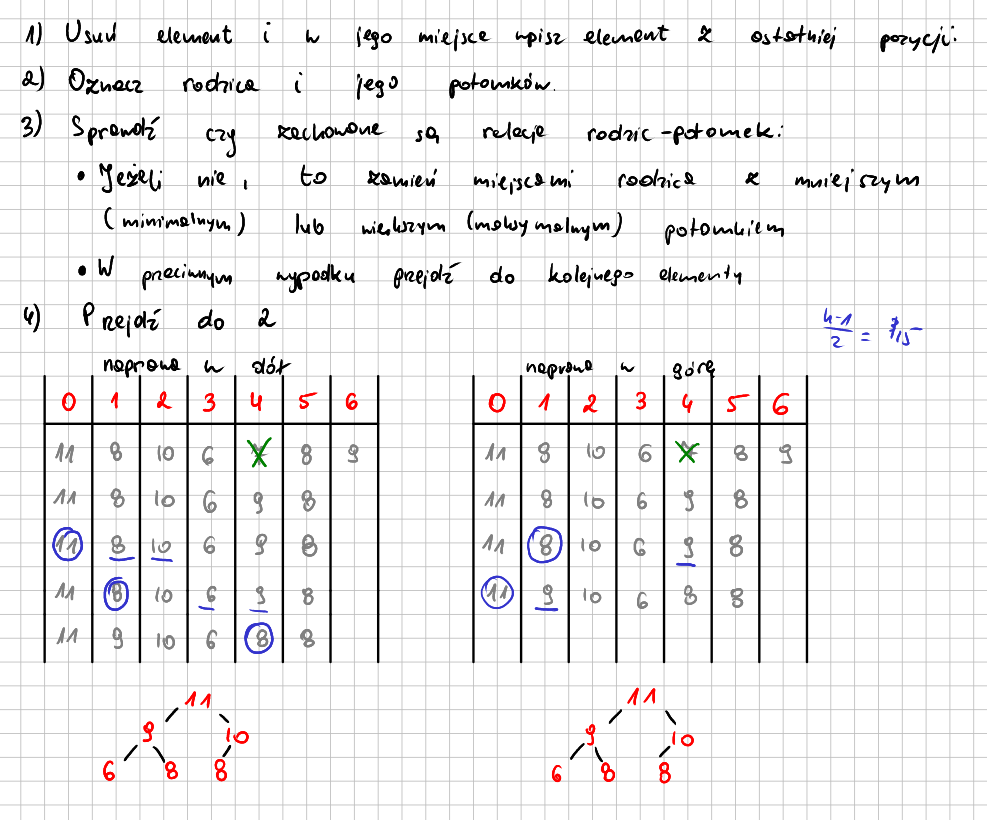
\includegraphics[width=14cm]{fig3.png}
\end{figure}

\newpage
\h{Algorytm naprawy kopca Floyda:}
\begin{figure}[H]
	\centering
	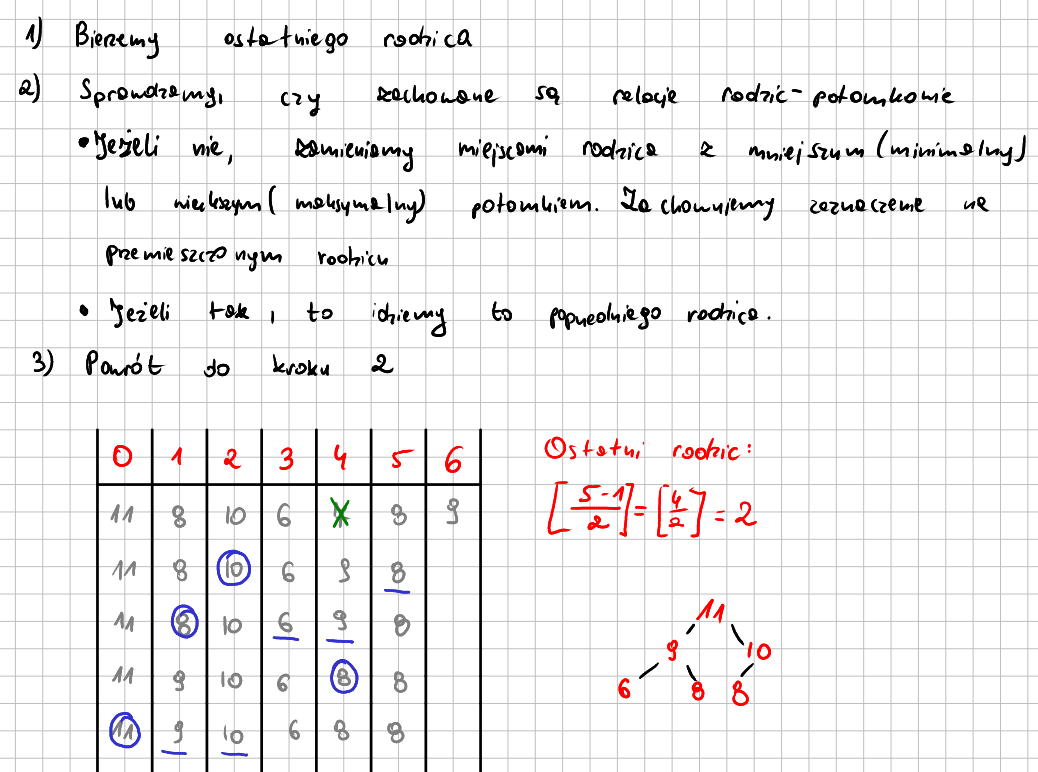
\includegraphics[width=14cm]{fig4.png}
\end{figure}


\end{document}